% Résumé du principe de l'expérience
Nous allons enregistré des vidéos d'un système munis de point de tracking tournant sous l'application d'une force constante, en faisant varier celle-ci et sa distance d'application. Les vidéos seront ensuite analysées afin d'obtenir l'accélération angulaire du système et observer le lien entre celle-ci et le moment de la force qui s'exerce sur le système.

\subsection{Matériel}
% Liste du matériel
Le matériel suivant est nécessaire afin de réaliser l'expérience:
\begin{multicols}{2}
\begin{itemize}
    \item Une soufflerie
    \item Un tube
    \item Un grand disque métallique
    \item 3 petits disques (diamètre de 3, 6 et 9 [$cm$])
    \item Une poulie
    \item Une ficelle
    \item Des poids (entre 20 et 90 [$g$])
    \item Un support de poids (10 [$g$])
    \item Du scotch
    \item Un stylo
    \item Du papier
    \item Un téléphone ou caméra
    \item Un statif
    \item Une plaque métallique
    \item Une noix de serrage
\end{itemize}
\end{multicols}

\subsection{Déroulement}
% Déroulement de l'expérience
Il est nécessaire d'assembler le dispositif d'expérimentation (voir figure \ref{fig:schm-glob}) avant les manœuvres suivantes. Il consiste en le grand disque métallique avec dessus les trois petits, autour desquels on peut entourer la ficelle, le tout monté sur un axe. On peut y scotcher un bout de papier avec un point noir au centre et un autre sur le bord afin de faire le tracking. On le met alors sur la soufflerie afin de réduire au maximum le frottement. De plus, on fixe une plaque métallique sur un statif afin de tenir le téléphone. Finalement, on aligne la poulie avec le bord des petits disque et on peut la fixer par exemple avec du scotch.\\ \\
Avant de commencer l'expérience, le téléphone doit être placé sur la planche métallique. L'entièreté du grand disque doit être inclue dans le cadrage et la soufflerie lancée (voir figure \ref{fig:schm-up}).

\subsubsection{Expérience 1}
\begin{enumerate}
    \item Lier une extrémité de le ficelle aux poids (30 [$g$] en plus du support) et faire passer celui-ci par la poulie.
    \item Enrouler l'autre extrémité de la ficelle autour l'un des trois petits disques.
    \item Commencer l'enregistrement de la vidéo.
    \item Donner un léger élan au grand disques pour enrouler le fil autour du disque. (Cela permet d'enregistrer l'accélération complète créé par la masse.)
    \item Une fois la masse descendue, arrêter l'enregistrement vidéo.
    \item Faire de même avec 50, 70 et 90 [g].
\end{enumerate}

\subsubsection{Expérience 2}
\begin{enumerate}
    \item Lier une extrémité de le ficelle aux poids (70 [$g$] avec le support) et faire passer celui-ci par la poulie.
    \item Enrouler l'autre extrémité de la ficelle autour du disque ayant un diamètre de 3 [$cm$].
    \item Commencer l'enregistrement de la vidéo.
    \item Donner un léger élan au grand disques pour enrouler le fil autour du disque. (Cela permet d'enregistrer l'accélération complète créé par la masse.)
    \item Une fois la masse descendue, arrêter l'enregistrement vidéo.
    \item Faire de même avec les disques de diamètre de 6 et 9 [$cm$].
\end{enumerate}

\subsection{Schémas}
% Schéma avec légende
\begin{minipage}{.5\textwidth}
\begin{figure}[H]
  \centering
    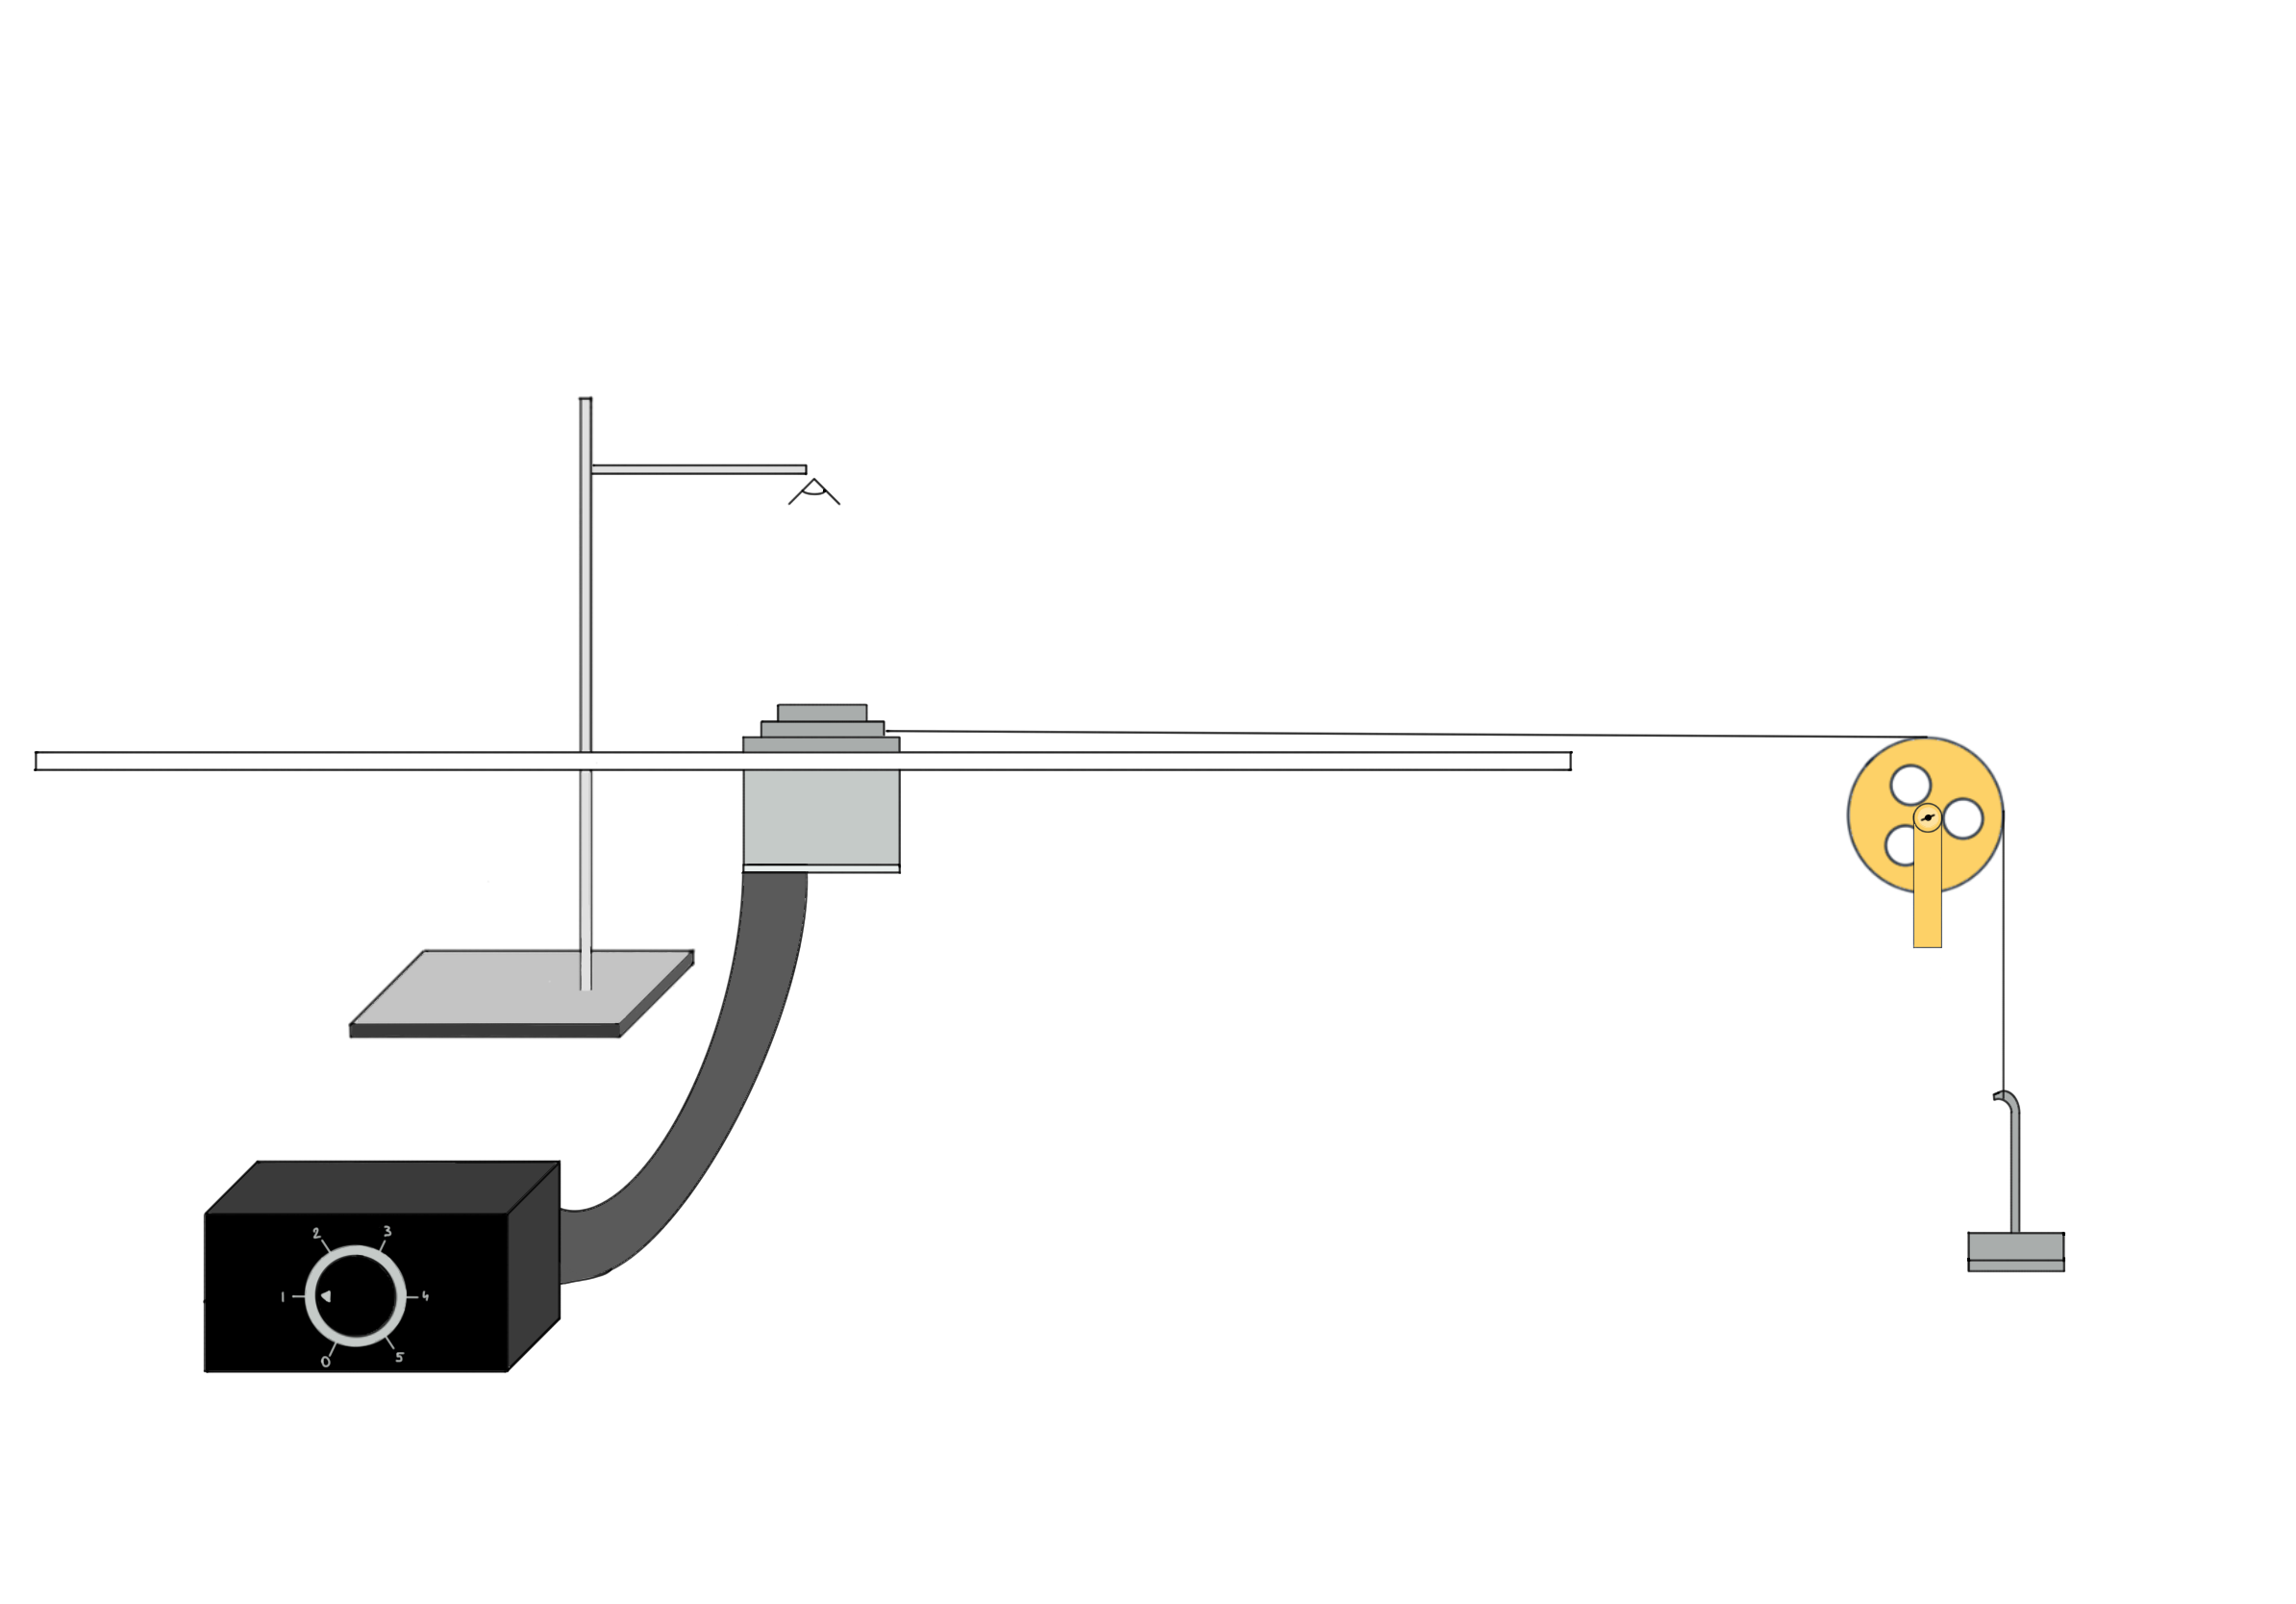
\includegraphics[width=1\textwidth]{Phy_rot1.png}
    \caption{Schéma de du dispositif d'expérimentation}
    \label{fig:schm-glob}
\end{figure}
\end{minipage}
\begin{minipage}{.5\textwidth}
\begin{figure}[H]
  \centering
    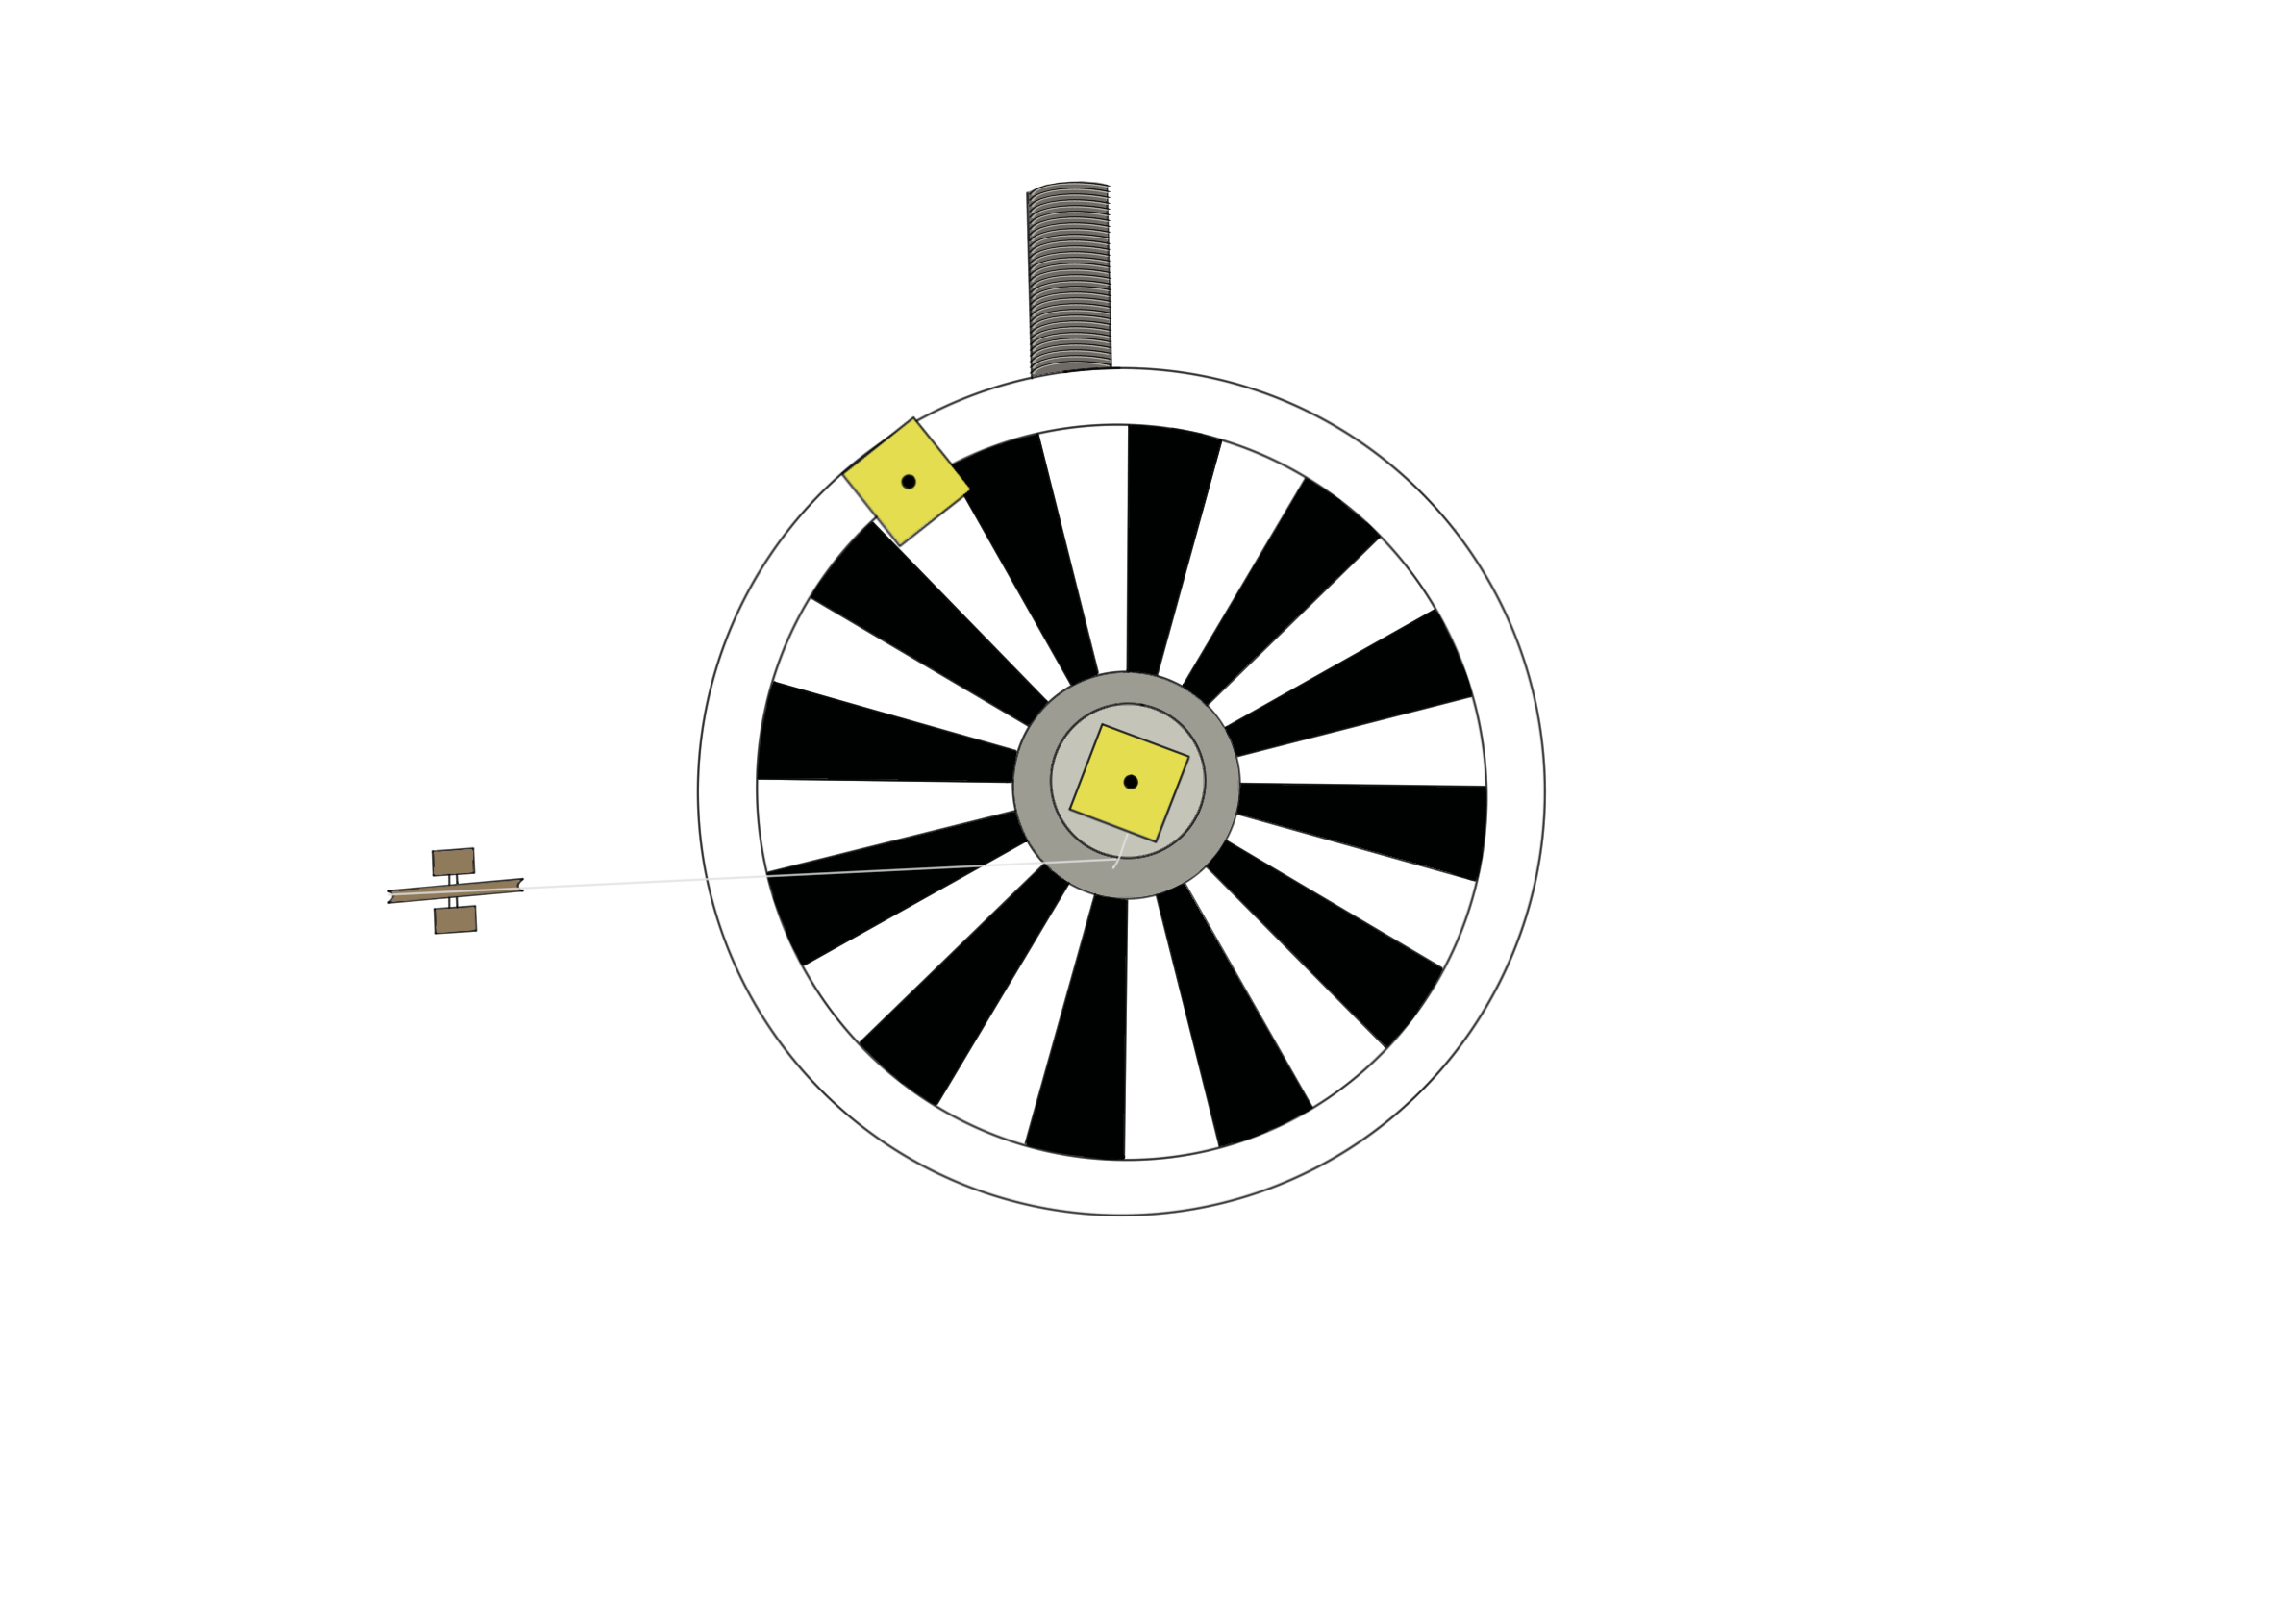
\includegraphics[width=1\textwidth]{Phy_rot2.png}
    \caption{Schéma des disques vus du dessus (point de vue de l'enregistrement vidéo)}
    \label{fig:schm-up}
\end{figure}
\end{minipage}
